\documentclass{article}

\usepackage{graphicx}

\title{Problem5 Report}
\author{Qi Liu}
\date{\today}

\begin{document}

\maketitle

\section{Overview}
All the figures below show the results.

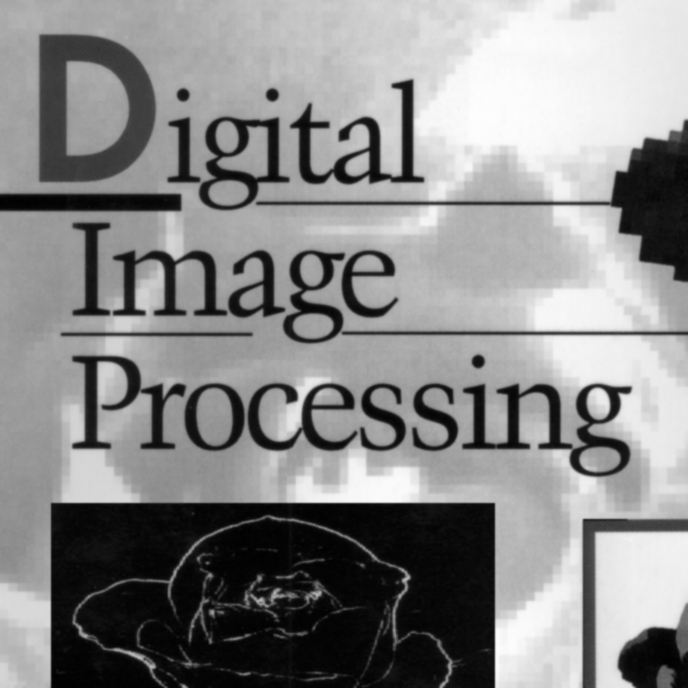
\includegraphics[width=0.25\textwidth]{../data/book_cover.jpg}
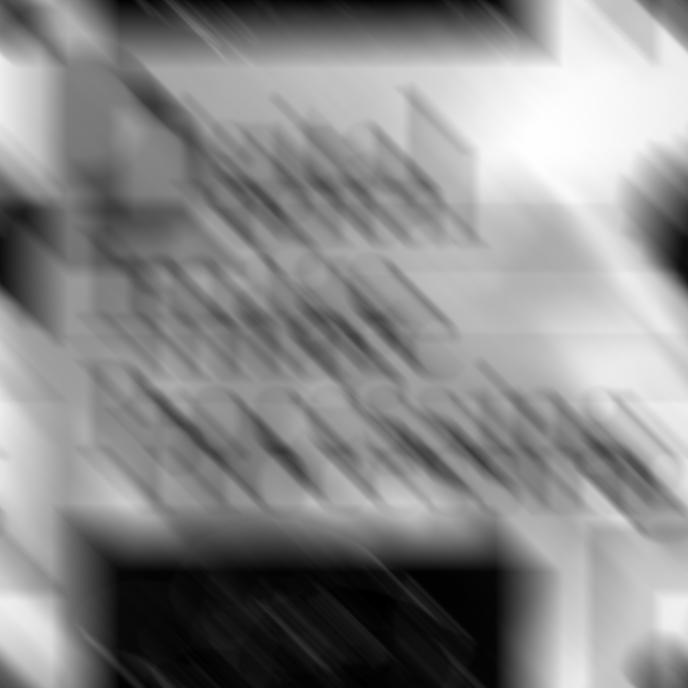
\includegraphics[width=0.25\textwidth]{../data/blur_0_book_cover.jpg}
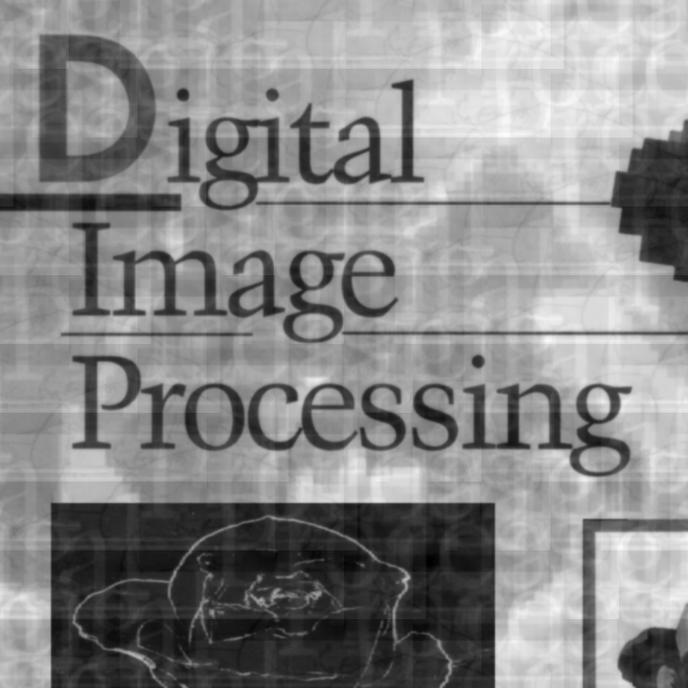
\includegraphics[width=0.25\textwidth]{../data/inverse_0_book_cover.jpg}
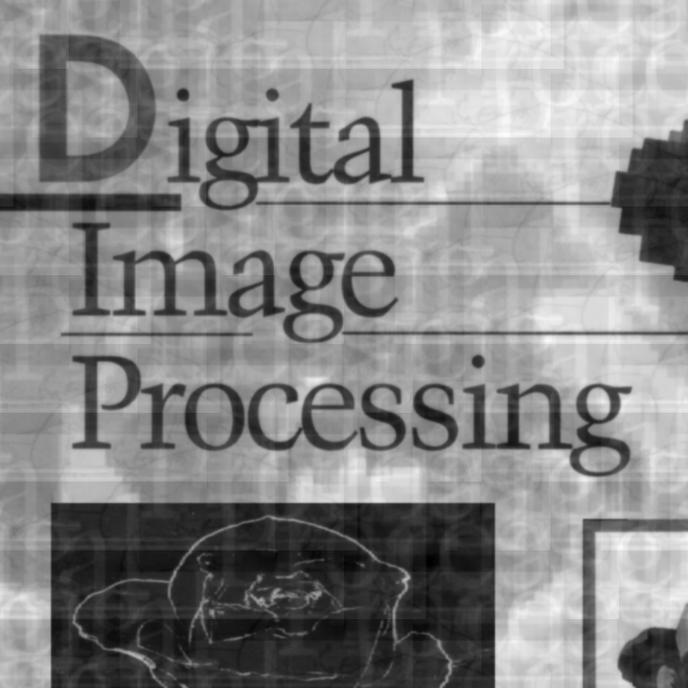
\includegraphics[width=0.25\textwidth]{../data/wiener_deconvolution_0_book_cover.jpg}

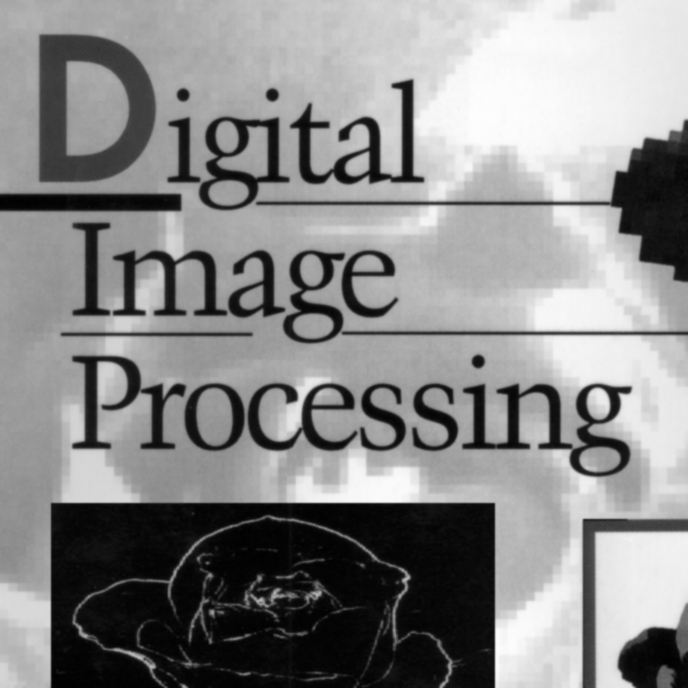
\includegraphics[width=0.25\textwidth]{../data/book_cover.jpg}
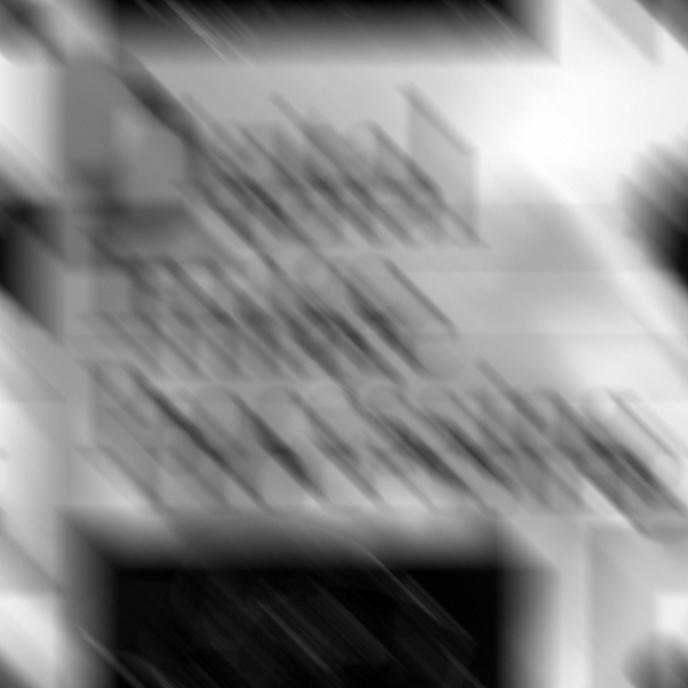
\includegraphics[width=0.25\textwidth]{../data/blur_1_book_cover.jpg}
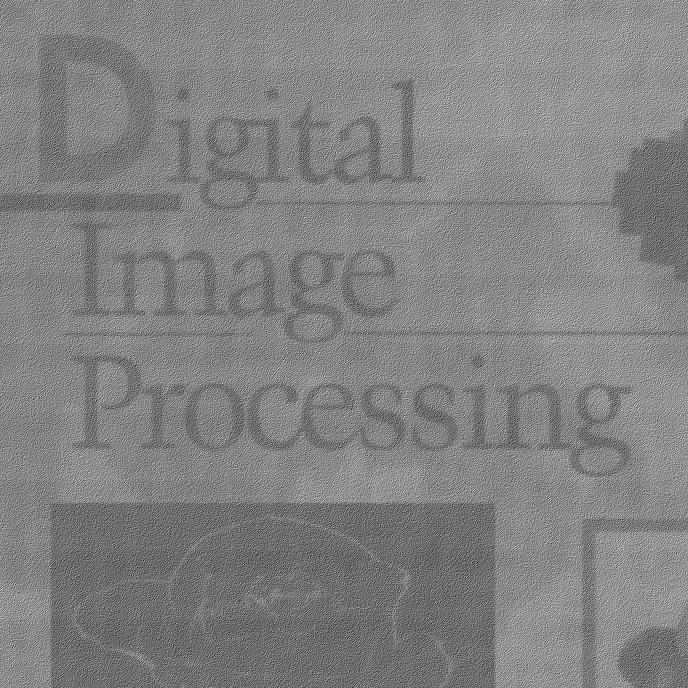
\includegraphics[width=0.25\textwidth]{../data/inverse_1_book_cover.jpg}
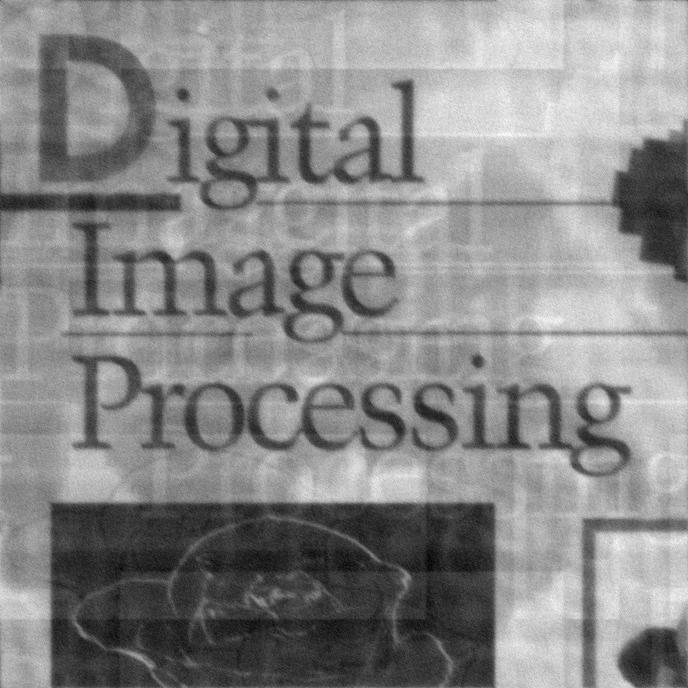
\includegraphics[width=0.25\textwidth]{../data/wiener_deconvolution_1_book_cover.jpg}

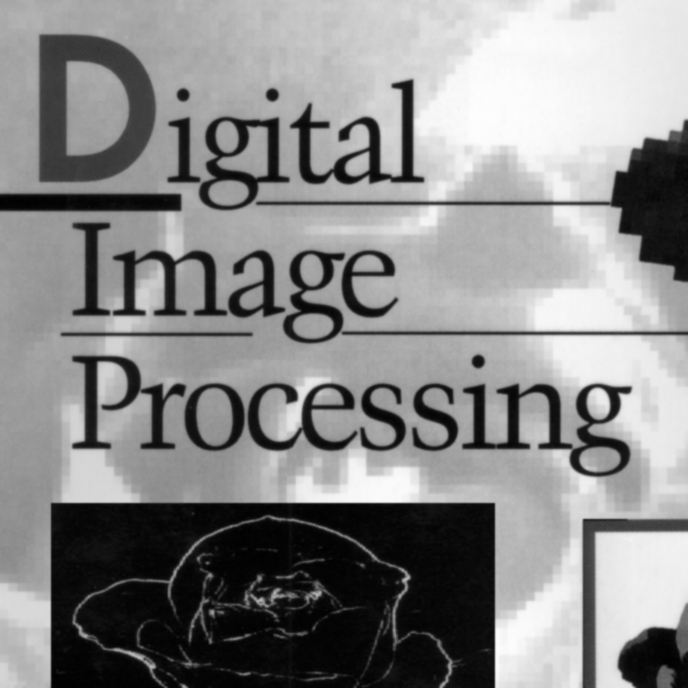
\includegraphics[width=0.25\textwidth]{../data/book_cover.jpg}
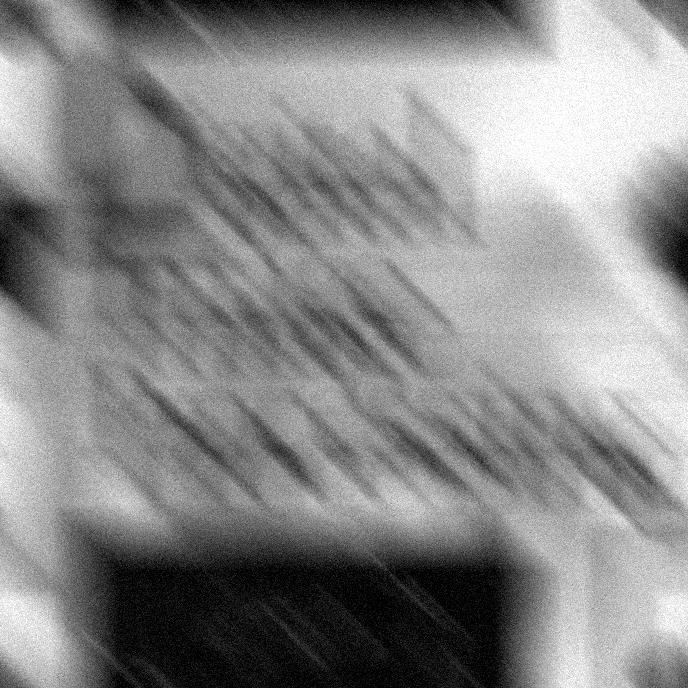
\includegraphics[width=0.25\textwidth]{../data/blur_150_book_cover.jpg}

\includegraphics[width=0.25\textwidth]{../data/inverse_150_book_cover.jpg}
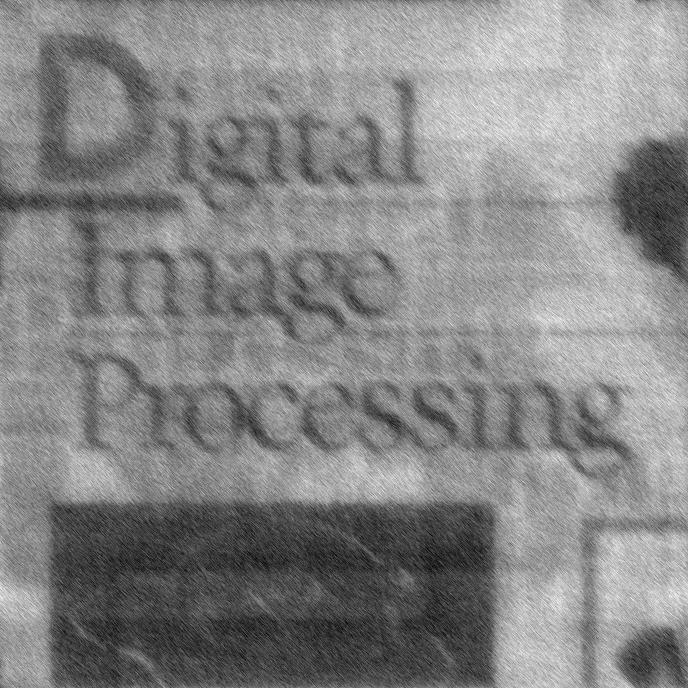
\includegraphics[width=0.25\textwidth]{../data/wiener_deconvolution_150_book_cover.jpg}

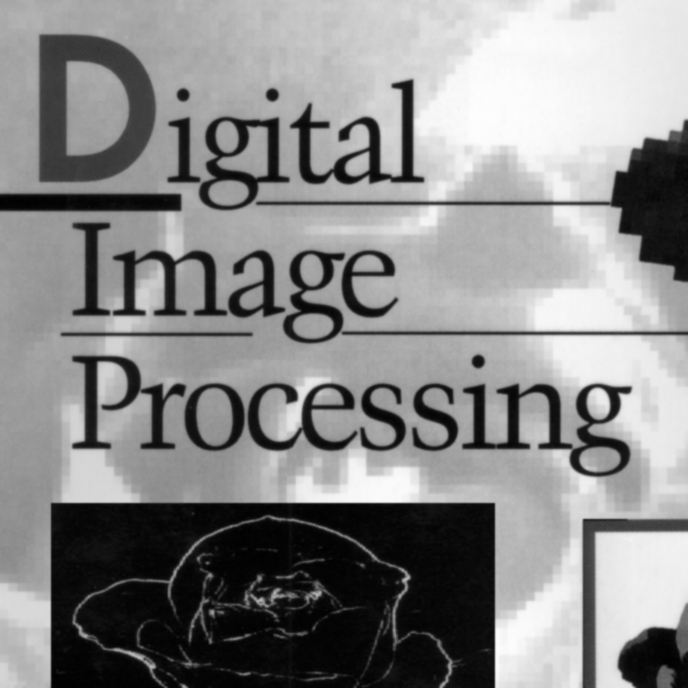
\includegraphics[width=0.25\textwidth]{../data/book_cover.jpg}
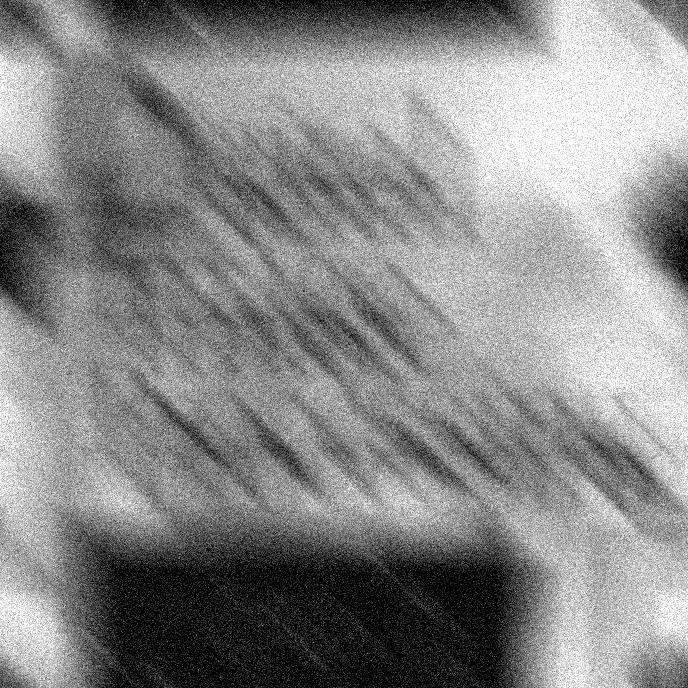
\includegraphics[width=0.25\textwidth]{../data/blur_650_book_cover.jpg}

\includegraphics[width=0.25\textwidth]{../data/inverse_650_book_cover.jpg}
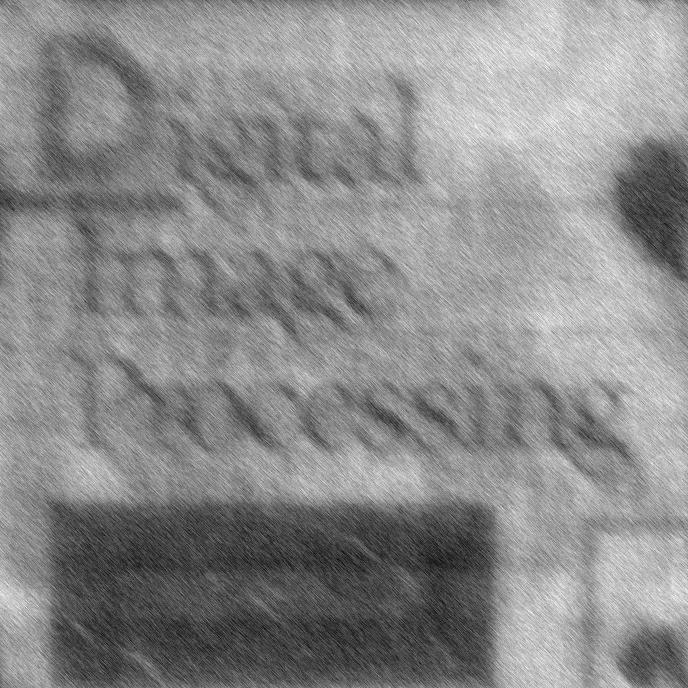
\includegraphics[width=0.25\textwidth]{../data/wiener_deconvolution_650_book_cover.jpg}

\section{Blurring Degradation Function}
The blurring degradation function we used is $$H(u,v)=\frac{T}{\pi(ua+vb)}\sin[\pi(ua+vb)]\exp[-j\pi(ua+vb)].$$ Here we set $a=b=0.1$ and $T=1$. The first column are the original images, the second column are the blurring images. The first row was not corrupted by any noises but the second to the fourth rows were corrupted by mean 0 Gaussian noises with variance 1, 150 and 650 respectively.

\section{Inverse Filter}
The inverse filter is just $$\hat{F}(u,v)=\frac{G(u,v)}{H(u,v)}.$$ The third column are the results of inverse filter. We can see its performance is good for the uncorrupted image (the result and the original image are a little different due to some float precision problems). But its performance is awful for the corrupted image. Even in the variance 1 case (in this case the blurring image has no visible noises), the texts are distinguishable but the noises are still visible in the result. In high variance cases, the results were dominated by the noises. 

\section{Wiener Deconvolution Filter}
We use approximated Wiener deconvolution filter $$\hat{F}(u,v)=[\frac{1}{H(u,v)}\frac{|H(u,v)|^2}{|H(u,v)|^2+K}]G(u,v).$$ The value K is manually set by 0, 0.001, 0.01 and 0.03 in the four cases respectively. The fourth column are the results of Wiener deconvolution filter. We can see its performance is better than inverse filter. Even in variance 650 case, the result is still distinguishable. 

\end{document}